\documentclass[,jou,floatsintext]{apa6}
\usepackage{lmodern}
\usepackage{amssymb,amsmath}
\usepackage{ifxetex,ifluatex}
\usepackage{fixltx2e} % provides \textsubscript
\ifnum 0\ifxetex 1\fi\ifluatex 1\fi=0 % if pdftex
  \usepackage[T1]{fontenc}
  \usepackage[utf8]{inputenc}
\else % if luatex or xelatex
  \ifxetex
    \usepackage{mathspec}
  \else
    \usepackage{fontspec}
  \fi
  \defaultfontfeatures{Ligatures=TeX,Scale=MatchLowercase}
\fi
% use upquote if available, for straight quotes in verbatim environments
\IfFileExists{upquote.sty}{\usepackage{upquote}}{}
% use microtype if available
\IfFileExists{microtype.sty}{%
\usepackage{microtype}
\UseMicrotypeSet[protrusion]{basicmath} % disable protrusion for tt fonts
}{}
\usepackage{hyperref}
\hypersetup{unicode=true,
            pdftitle={Justify Your Alpha: A Practical Guide},
            pdfauthor={Daniël Lakens},
            pdfkeywords={hypothesis testing, Type 1 error, Type 2 error, statistical power},
            pdfborder={0 0 0},
            breaklinks=true}
\urlstyle{same}  % don't use monospace font for urls
\usepackage{graphicx,grffile}
\makeatletter
\def\maxwidth{\ifdim\Gin@nat@width>\linewidth\linewidth\else\Gin@nat@width\fi}
\def\maxheight{\ifdim\Gin@nat@height>\textheight\textheight\else\Gin@nat@height\fi}
\makeatother
% Scale images if necessary, so that they will not overflow the page
% margins by default, and it is still possible to overwrite the defaults
% using explicit options in \includegraphics[width, height, ...]{}
\setkeys{Gin}{width=\maxwidth,height=\maxheight,keepaspectratio}
\IfFileExists{parskip.sty}{%
\usepackage{parskip}
}{% else
\setlength{\parindent}{0pt}
\setlength{\parskip}{6pt plus 2pt minus 1pt}
}
\setlength{\emergencystretch}{3em}  % prevent overfull lines
\providecommand{\tightlist}{%
  \setlength{\itemsep}{0pt}\setlength{\parskip}{0pt}}
\setcounter{secnumdepth}{0}
% Redefines (sub)paragraphs to behave more like sections
\ifx\paragraph\undefined\else
\let\oldparagraph\paragraph
\renewcommand{\paragraph}[1]{\oldparagraph{#1}\mbox{}}
\fi
\ifx\subparagraph\undefined\else
\let\oldsubparagraph\subparagraph
\renewcommand{\subparagraph}[1]{\oldsubparagraph{#1}\mbox{}}
\fi

%%% Use protect on footnotes to avoid problems with footnotes in titles
\let\rmarkdownfootnote\footnote%
\def\footnote{\protect\rmarkdownfootnote}


  \title{Justify Your Alpha: A Practical Guide}
    \author{Daniël Lakens\textsuperscript{1}}
    \date{}
  
\shorttitle{Justify in Practice}
\affiliation{
\vspace{0.5cm}
\textsuperscript{1} Eindhoven University of Technology, The Netherlands}
\keywords{hypothesis testing, Type 1 error, Type 2 error, statistical power\newline\indent Word count: XXXX words.}
\usepackage{csquotes}
\usepackage{upgreek}
\captionsetup{font=singlespacing,justification=justified}

\usepackage{longtable}
\usepackage{lscape}
\usepackage{multirow}
\usepackage{tabularx}
\usepackage[flushleft]{threeparttable}
\usepackage{threeparttablex}

\newenvironment{lltable}{\begin{landscape}\begin{center}\begin{ThreePartTable}}{\end{ThreePartTable}\end{center}\end{landscape}}

\makeatletter
\newcommand\LastLTentrywidth{1em}
\newlength\longtablewidth
\setlength{\longtablewidth}{1in}
\newcommand{\getlongtablewidth}{\begingroup \ifcsname LT@\roman{LT@tables}\endcsname \global\longtablewidth=0pt \renewcommand{\LT@entry}[2]{\global\advance\longtablewidth by ##2\relax\gdef\LastLTentrywidth{##2}}\@nameuse{LT@\roman{LT@tables}} \fi \endgroup}

\authornote{All code used to create this manuscript is provided in an OSF repository at \url{https://osf.io/xxxxx/}.

Correspondence concerning this article should be addressed to Daniël Lakens, ATLAS 9.402, 5600 MB, Eindhoven, The Netherlands. E-mail: \href{mailto:D.Lakens@tue.nl}{\nolinkurl{D.Lakens@tue.nl}}}

\abstract{
Justify Everything.


}

\begin{document}
\maketitle

Researchers often rely on data to decide how to act. In a Neyman-Pearson approach to hypothesis testing (Neyman \& Pearson, 1933) studies are designed such that erroneous decisions that determine how we act are controlled in the long run at some desired maximum level. If resources were infinite we could collect so much data that the chance of making a wrong decision is incredibly small. But resources are often limited, which means that researchers need to decide how to choose the rate at which they are willing to make errors. After data is collected researchers can incorrectly act as if there is an effect when there is no true effect (a Type 1 error) or incorrectly act as if there is no effect when there is a true effect (a Type 2 error). For any fixed sample size and true effect size a reduction in the Type 1 error rate will increase the Type 2 error rate and vice versa.

The question how error rates should be set in any study requires careful consideration of the relative costs of a Type 1 error or a Type 2 error. Regrettably researchers rarely provide such a justification, and predominantly use a Type 1 error rate of 5\%. One reason researchers predominantly rely on norms instead of rationally chosen error rates is the absence of explanations how to justify a different alpha level than the normative use of 0.05. In this article I will explain why error rates need to be justified, and will provide two practical guidelines that can be used to justify the alpha level based on the sample size, or to balance or minimize the type 1 and Type 2 error rate.

\hypertarget{why-do-we-use-a-5-alpha-level-and-80-power}{%
\section{Why do we use a 5\% alpha level and 80\% power?}\label{why-do-we-use-a-5-alpha-level-and-80-power}}

As a young scholar we might naively assume that when all researchers do something, there must be a good reason for such an established practice. An important step towards maturity as a scholar is the realization that this is not the case. Neither Fisher nor Neyman, two statistical giants largely responsible for the widespread reliance on hypothesis tests in the social sciences, recommended the universal use of any specific threshold. Fisher (1935) writes: \enquote{It is open to the experimenter to be more or less exacting in respect of the smallness of the probability he would require before he would be willing to admit that his observations have demonstrated a positive result.} Similarly, Neyman and Pearson (1933) writes: \enquote{From the point of view of mathematical theory all that we can do is to show how the risk of the errors may be controlled and minimized. The use of these statistical tools in any given case, in determining just how the balance should be struck, must be left to the investigator.}

Even though in theory alpha levels should be justified, in practice researchers tend to imitate others. Fischer writes in 1926: \enquote{Personally, the writer prefers to set a low standard of significance at the 5 per cent point, and ignore entirely all results which fail to reach this level}. This sentence is preceded by the statement \enquote{If one in twenty does not seem high enough odds, we may, if we prefer it, draw the line at one in fifty (the 2 percent point), or one in a hundred (the 1 percent point).} Indeed, in his examples Fisher often uses an alpha of 0.01. Nevertheless, researchers seem to have copied the value Fisher preferred, instead of his more important take-home message that the significance level should be set by the experimenter. The default use of an alpha level of 0.05 by seems to originate from the early work of Gosset on the \emph{t}-distribution (Cowles \& Davis, 1982), who believed that a deviation of two standard deviations (a z-score of 2) was sufficiently rare.

The default use of 80\% power (or a 20\% Type 2, or beta (b) error) is similarly based on personal preferences by Cohen (1988), who writes: \enquote{It is proposed here as a convention that, when the investigator has no other basis for setting the desired power value, the value .80 be used. This means that b is set at .20. This arbitrary but reasonable value is offered for several reasons (Cohen, 1965, pp.~98-99). The chief among them takes into consideration the implicit convention for a of .05. The b of .20 is chosen with the idea that the general relative seriousness of these two kinds of errors is of the order of .20/.05, i.e., that Type I errors are of the order of four times as serious as Type II errors. This .80 desired power convention is offered with the hope that it will be ignored whenever an investigator can find a basis in his substantive concerns in his specific research investigation to choose a value ad hoc.}

Ironically, we see that the norm to aim for 80\% power is built on the norm to set the alpha level at 5\%. If we ignore this slightly depressing practice of building conventions upon conventions, the real lesson Cohen was teaching us was to determine the relative seriousness of a Type 1 and Type 2 error, and balancing both types of errors when a study is designed. If a Type 1 error is considered to be four times as serious as a Type 2 error, the \emph{weighted} error rates in the study are balanced. Instead of imitating the value chosen by Cohen, researchers should aim to imitate the approach he used to justify error rates.

\hypertarget{why-error-rates-should-be-justified}{%
\subsection{Why error rates should be justified}\label{why-error-rates-should-be-justified}}

In 1957 Neyman wrote: \enquote{it appears desirable to determine the level of significance in accordance with quite a few circumstances that vary from one particular problem to the next.} Despite this good advice, social scientists developed the norm to always use an alpha level of 0.05 as a significance threshold when testing hypotheses, and aim for a minimum (and thereby default) power of 0.80. This mindless use of null hypothesis significance test has been criticized for more than half a century (Bakan, 1966; Gigerenzer, 2018), but there have been few attempts to provide researchers with practical guidelines to do anything else than blindly following norms. It is difficult to abandon a mediocre research practice without an alternative.

There are two main reasons to abandon the universal use of a 5\% alpha level. The first reason to carefully choose an alpha level is that decision making becomes more efficient. If researchers use hypothesis tests to choose how to act while balancing error rates it is typically possible to make decisions more efficiently by setting a different alpha level than 0.05. If we aim to either minimize or balance Type 1 and Type 2 error rates for a given sample size and effect size, the alpha level should be set not based on convention, but by weighting the relative costs of both types of errors.

The second reasons is that as the statistical power increases, some \emph{p}-values below 0.05 (e.g., \emph{p} = 0.04) can be more likely when there is no effect than when there is an effect. This is known as Lindley's paradox (see Lindley (1957) Cousins (2017)). The distribution of \emph{p}-values is a function of the statistical power (Cumming, 2008), and the higher the power, the more right-skewed the distribution becomes (i.e.~the more low \emph{p}-values are observed). When there is no true effect \emph{p}-values are uniformly distributed, and 1\% of observed \emph{p}-values fall between 0.04 and 0.05. When the statistical power is extremely high, not only will most \emph{p}-values fall below 0.05, most will also fall below 0.01. In Figure \ref{fig:p-plot} we see that with high power very low \emph{p}-values are more likely to be observed when there \emph{is} an effect than when there is \emph{no} effect (e.g., the black curve representing \emph{p}-values when the alternative is true falls above the dashed horizontal line for a \emph{p}-value of 0.01). But observing a \emph{p}-value of 0.04 is more likely when the null hypothesis is true than when the alternative hypothesis is true and we have very high power (the horizontal dashed line falls above the black curve for \emph{p}-values larger than \textasciitilde0.025).

\begin{figure}
\centering
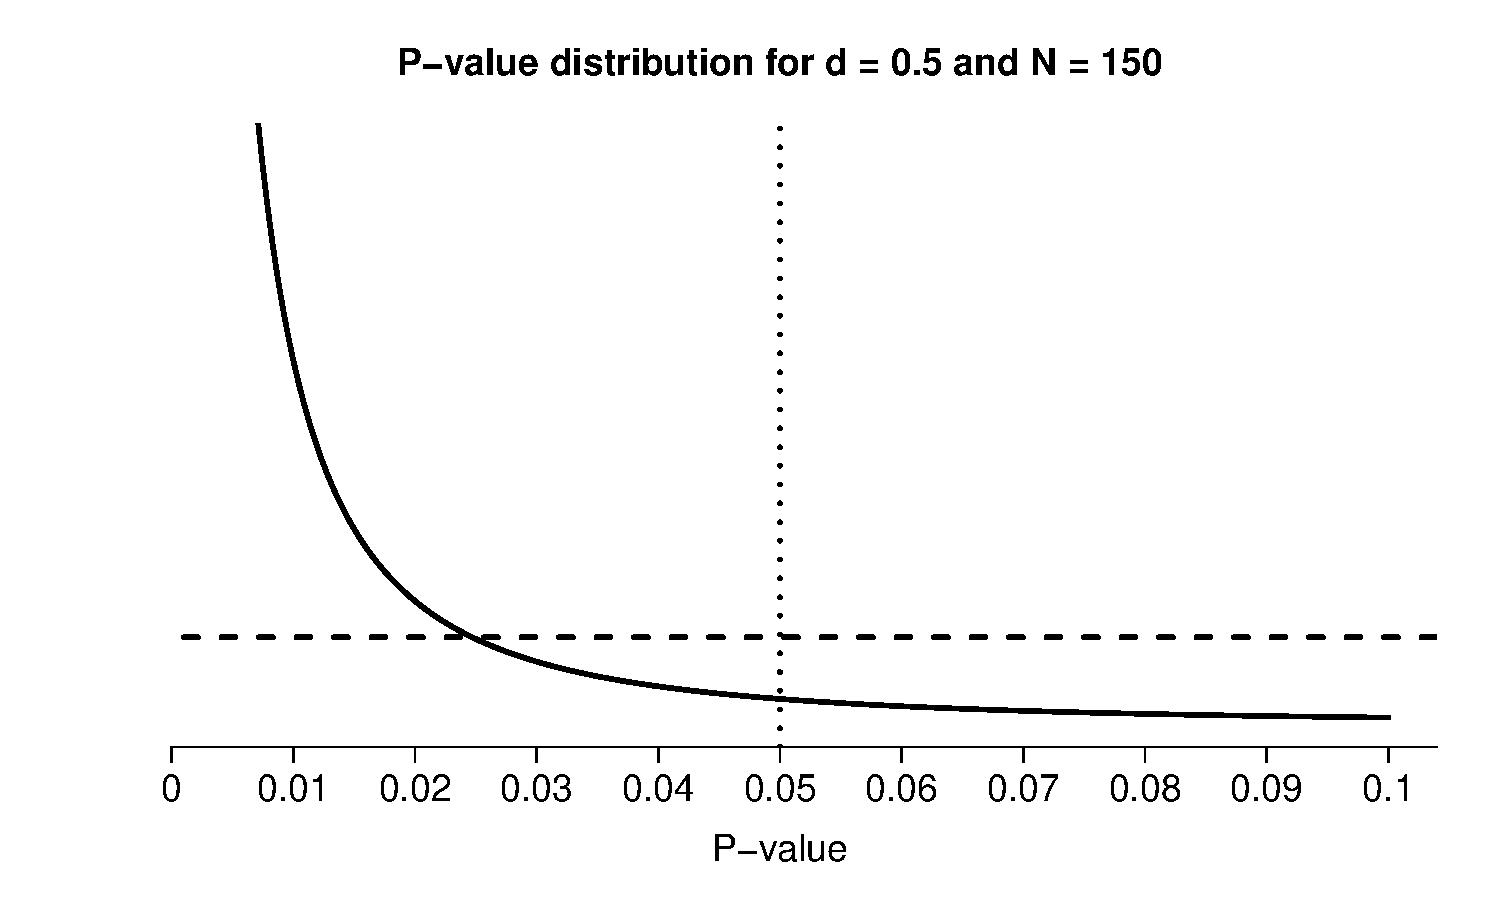
\includegraphics{Justify_in_Practice_files/figure-latex/p-plot-1.pdf}
\caption{\label{fig:p-plot}\emph{P}-value distributions for a two-sided independent \emph{t}-test with N = 150 and d = 0.5 (black curve) or d = 0 (horizontal dashed line).}
\end{figure}

Researchers often want to interpret a significant test result as \enquote{support} for the alternative hypothesis. If so, it makes sense to choose the alpha level such that when a significant \emph{p}-value is observed, the \emph{p}-value is actually more likely when the alternative hypothesis is true than when the null hypothesis is true. This means that when statistical power is very high (e.g., the sample size is very large), the alpha level should be reduced. If the alpha level in Figure \ref{fig:p-plot} is lowered to 0.02 then the alternative hypothesis is more likely than the null hypothesis for all significant \emph{p}-values that would be observed.

\hypertarget{minimizing-or-balancing-type-1-and-type-2-error-rates}{%
\subsection{Minimizing or Balancing Type 1 and Type 2 Error Rates}\label{minimizing-or-balancing-type-1-and-type-2-error-rates}}

If both Type 1 as Type 2 errors are costly, then it makes sense to optimally reduce both errors as you design studies. This would make decision making overall most efficient. Researchers can choose to design a study with a statistical power and alpha level that minimize the \emph{combined error rate}. For example, with a 5\% alpha level and a statistical power of 80\% the combined error rate is 5 + 20 = 25\%. If the statistical power is 99\% and the alpha is 5\% the combined error rate is 1 + 5 = 6\%. Mudge, Baker, Edge, and Houlahan (2012) show that by choosing an alpha level based on the relative weight of Type 1 errors and Type 2 errors, and if desired beliefs about the prior probability that H0 and H1 are true, decision making can be more efficient than when relying on the default alpha level of 0.05.

Winer (1962) writes: \enquote{The frequent use of the .05 and .01 levels of significance is a matter of convention having little scientific or logical basis. When the power of tests is likely to be low under these levels of significance, and when type 1 and type 2 errors are of approximately equal importance, the .30 and .20 levels of significance may be more appropriate than the .05 and .01 levels.} The reasoning here is that a design that has 70\% power for the smallest effect size of interest would not balance the Type 1 and Type 2 error rates in a sensible manner. Similarly, in huge datasets it might be possible to achieve very high levels of power for all effect sizes that are still considered meaningful, and a study design which has 99\% power but uses a 5\% alpha level similarly suffers from a lack of balance. A common example is a meta-analysis, which often have extremely high power for any effect size that would be considered meaningful, but where researchers often use a 5\% Type 1 error rate anyway.

Researchers can decide to either balance Type 1 and Type 2 error rates (e.g., setting both at 5\%), or minimize error rates. For any given sample size and effect size one wants to detect, there is an alpha level that minimizes the combined error rates. Because the alpha level also influences the statistical power and thus the Type 2 error rate and iterative procedure is needed that determines the optimal value for the alpha level. For example, for a study which will be analyzed with an independent two-sided t-test with n = 64 per condition, and an effect size that the researchers wants to detect of d = 0.5, the combined error rate is minimized when \(\alpha\) = 0.0997 and the Type 2 error rate \(\beta\) = 0.122. For the same scenario, balanced error rates are \(\alpha\) = 0.111 and \(\beta\) = 0.111.

\hypertarget{weighing-the-relative-cost-of-errors}{%
\subsubsection{Weighing the relative cost of errors}\label{weighing-the-relative-cost-of-errors}}

Cohen (1988) considered a Type 1 error rate of 5\% and a Type 2 error rate balanced. The reason for this was that instead of weighing both types of errors equally, he felt \enquote{Type I errors are of the order of four times as serious as Type II errors}. To determine the relative costs of Type 1 and Type 2 errors researchers should perform a cost-benefit analysis. Although it can be difficult to formally quantify all factors that determine the costs of Type 1 and Type 2 errors, there is no reason to let the perfect be the enemy of the good, and in many research questions where there are no direct applications of the research findings, relative costs might be largely subjective.

If we adapt our calculations for the \emph{t}-test above, with d = 0.5, n = 64, but now weigh the cost of Type 1 errors 4 times as much as Type 2 errors, balanced error rates are \(\alpha\) = 0.0498 and \(\beta\) = 0.199. You personally might believe the cost of a Type 1 error is only twice as severe as a Type 2 error, in which case balanced error rates would mean designing a study with \(\alpha\) = 0.0754 and \(\beta\) = 0.151.

\hypertarget{incorporating-prior-probabilities}{%
\subsubsection{Incorporating prior probabilities}\label{incorporating-prior-probabilities}}

Miller and Ulrich (2019) explain how the choice for an optimal alpha level depends not just on the relative costs of Type 1 and Type 2 errors, but also on the base rate of true effects. In the extreme case, if all studies a researcher designs test true hypotheses there is no reason to worry about Type 1 errors (because the null hypothesis is never true, you can never conclude there is an effect when there is no effect) and you can set the alpha level to 1. If the base rate of true hypotheses is very low, in the long run you will make many more Type 1 errors than Type 2 errors. For example, if you perform 1000 studies, and the base rate of true effects is 10\%, with 5\% Type 1 error rate and a 5\% Type 2 error rate you will observe 1000 × 0.1 × 0.05 = 5 Type 2 errors, and 1000 × 0.9 × 0.05 = 45 Type 1 errors. The long run frequency of Type 1 errors and Type 2 errors is not balanced in this example.

If you want to balance or minimize error rates in the long run, you should lower the alpha level as a function of the base rate of true hypotheses. Because the base rate of true hypotheses is unknown, this step requires subjective judgment. This can not be avoided, because one always makes assumptions about base rates, even if this assumption is that a hypothesis is equally likely to be true as false (a ratio of H1/H0 of 1/1 = 1). Assuming equal prior probabilities for H1 and H0, we saw above that balanced error rates assuming d = 0.5 and collection n = 64 per condition in a \emph{t}test would imply \(\alpha\) = 0.111 and \(\beta\) = 0.111. If you assume it is ten times as likely that the null hypothesis is true than that the alternative hypothesis is true (a ratio of H1/H0 of 1/10 = 0.1) balanced error rates would require setting \(\alpha\) = 0.0275 and \(\beta\) = 0.275. If you believe the alternative hypothesis is twice as likely to be true than the null hypothesis, balancing error rates in the long run would mean increasing the alpha level and increasing the power by choosing \(\alpha\) = 0.159 and \(\beta\) = 0.0795.

To minimize the combined error rates Equation \eqref{eq:minimize} needs to be minimize the \(\alpha\) and \(\beta\), which requires an iterative procedure since the power, or 1-\(\beta\), also depends on the \(\alpha\) level. When balancing error rates the difference between the \(\alpha\) and \(\beta\) is minimized in an iterative procedure. Both approaches typicaly yield quite similar resuls. Where minimizing error rates might be slightly more efficient, balancing error rates might be slightly more intuitive (especially when the prior probability of H0 and H1 are equal).

\begin{equation}
\frac{(cost_{T1T2} \times \alpha + prior_{H1H0} \times \beta)}{prior_{H1H0}+1}
\label{eq:minimize}
\end{equation}

\hypertarget{lowering-the-alpha-level-as-a-function-of-the-sample-size}{%
\subsection{Lowering the Alpha Level as a Function of the Sample Size}\label{lowering-the-alpha-level-as-a-function-of-the-sample-size}}

Sometimes it is difficult to make a statement about the power (and hence the Type 2 error rate) of the statistical test. Calculating the power requires specifying the alternative hypothesis: Which effect sizes does the theory predict, or is the smallest effect size of interest. In these cases there is a less philosophically coherent approach to justifying the apha level that, although basically a heuristic in itself, is nevertheless an improvement over current practices. It is offered here in the spirit of not making the perfect the enemy of the good. Whenever is it too difficult to make a statement about the power of the test, and a researcher is tempted to fall back to the norm to use an alpha level of 0.05, it is still an improvement to lower the alpha level as a function of the sample size.

This approach is discussed most extensively by Leamer (1978). He writes \enquote{The rule of thumb quite popular now, that is, setting the significance level arbitrarily to .05, is shown to be deficient in the sense that from every reasonable viewpoint the significance level should be a decreasing function of sample size.} This was already recognized by Jeffreys (1939), who discusses ways to set the alpha level in Neyman-Pearson statistics: \enquote{We should therefore get the best result, with any distribution of alpha, by some form that makes the ratio of the critical value to the standard error increase with n.~It appears then that whatever the distribution may be, the use of a fixed P limit cannot be the one that will make the smallest number of mistakes.}

To understand this recommendation it is important to distinguish between statistical inferences based on error control and inferences based on likelihoods. When the alpha level is set to 5\% a researcher will not conclude there is an effect when there is no true effect more than 5\% of the time (in the long run, and when all test assumptions hold). However, from a likelihood perspective it is possible that the observed data is much more likely when the null hypothesis is true, than when the alternative hypothesis is true, even when the observed \emph{p}-value is smaller than 0.05. As explained in Figure \ref{fig:p-plot} this is known as Lindley's paradox. In Bayesian statistics Lindley's paradox is prevented because the critical value does not approach a limit as the sample size increases (i.e., a critical value of 1.96 for \emph{p} = 0.05 in a two-sided test). Instead, the same Bayes factor corresponds to a larger test statistic as the sample size increases (see Rouder, Speckman, Sun, Morey, and Iverson (2009) and Zellner (1971)).

To prevent Lindley's paradox one would need to lower the alpha level as a function of the statistical power. Good (1992) notes: \enquote{we have empirical evidence that sensible \emph{P} values are related to weights of evidence and, therefore, that \emph{P} values are not entirely without merit. The real objection to \emph{P} values is not that they usually are utter nonsense, but rather that they can be highly misleading, especially if the value of N is not also taken into account and is large.} Based on the observation by Jeffrey's (1939) that, under specific circumstances, the Bayes factor against the null hypothesis is approximately inversely proportional to (\(\sqrt{N}\)), Good (1982) suggests a standardized \emph{p}-value to bring \emph{p}-values in closer relationship with weights of evidence:
\begin{equation}
p_{stan} = p\sqrt{\frac{N}{100}} 
\label{eq:pstan}
\end{equation}
where \emph{p} is the observed \emph{p}-value and \emph{N} is the total sample size. This formula standardizes the \emph{p}-value to the evidence against the null hypothesis that would be observed if \(p_{stan}\) was the tail area probability observed in a sample of 100 participants. It is perhaps easier to think about a standardized alpha level:
\begin{equation}
\alpha_{stan} = \frac{\alpha}{\sqrt{\frac{N}{100}}} \label{eq:astan}
\end{equation}

With 100 participants \(\alpha\) and \(\alpha_{stan}\) are the same, but as the sample size increases beyond 100 observations the alpha level decreases. A higher critical test-statistic needs to be observed to still consider a finding \enquote{statistically significant} as the sample size increases, which prevents Lindley's paradox. For example, an \(\alpha\) = 0.05 for a sample size of 500 would become an \(\alpha_{stan}\) of 0.022.

As mentioned by Rouder et al. (2009): \enquote{NP testing can be made consistent by allowing Type I error rates to decrease toward zero as the sample size increases. How this rate should decrease with sample size, however, is neither obvious nor stipulated by the statistical theory underlying NP testing.} Indeed, whereas lowering the alpha level as the sample size increases is a valid approach, the specific way to do this as proposed by Good (1982) is itself largely based on the heuristic that starting to lower the alpha level when the number of total observations increases above 100 is largely a heuristic. There is no special reason to standardize the \emph{p}value or alpha level to 100 observations, or to choose a 5\% alpha level as a starting point. The reason to nevertheless recommend this justification for the alpha level is that it is straightforward to implement and is, despite the rather random choice of N = 100, in practice most likely quite succesful in preventing Lindley's paradox for most studies in psychology.

There are other ways to calibrate \emph{p}-values so that they are more in line with Bayes factors (see Sellke, Bayarri, and Berger (2001) and Benjamin et al. (2018)), but not everyone thinks such calibrations are sensible (Senn, 2001). Researchers might want to report \enquote{a B for every \emph{p}}, or a Bayes factor for every \emph{p}-value (Dienes \& Mclatchie, 2017), and take any disagreement between these two approaches (which should be quite rare according to Jeffreys, 1939) as a reason to be cautious when drawing conclusions from the data.

\hypertarget{discussion}{%
\section{Discussion}\label{discussion}}

Editors and reviewers should \emph{always} ask authors to justify their choice of error rates, whenever researchers use data to make decisions about the presence or absence of an effect. As Skipper, Guenther, and Nass (1967) remarks: \enquote{If, in contrast with present policy, it were conventional that editorial readers for professional journals routinely asked:}What justification is there for this level of significance?" authors might be less likely to indiscriminately select an alpha level from the field of popular eligibles." Reviewers and editors who embrace this recommendation should expect some annoyance. It is often confronting to be asked to justify a norm you have taken for granted your entire life, only to realize you don't have any justification.

If a power analysis can be performed (i.e., whenever a desired or expected effect size of interest can be specified) researchers could do much worse than to design a study such that the combined error rate is minimized or balanced. If it is difficult to specify an effect size of interest (and thus to perform an a-priori power analysis and calculate a Type 2 error rate) researchers can fall back to the approach where the alpha level is reduced as a function of the sample size.

I have created a Shiny app that allows users to perform the calculations recommended in this article. It allows users to to minimize \(\alpha\) and \(\beta\) (or their difference), which works by specifying the effect size and sample size, as well as an analytic power calculation. The effect size should be determined as in a normal power analysis (preferably based on the smallest effect size of interest, for recommendations, see Albers and Lakens (2018)), and the sample size can be increased until the error rates are deemed acceptable. Alternatively, researchers lower the alpha level as a function of the sampe size by spacifying their sample size. Whichever approach is used, it is strongly recommended to preregister the alpha level that researchers plan to use before the data is collected.

Because of the strong overreliance on a 5\% error rate when designing studies, we have seen relatively few people attempt to justify their alpha level. Examples in other research domains exist. For example, Field, Tyre, Jonzén, Rhodes, and Possingham (2004) quantify the relative costs of Type 1 errors when testing whether native species in Australia are declining. They come to the conclusion that when it comes to the Koala population, given its great economic value, the alpha level should be set to 1. In other words, one should always act as if the population is declining, because the relative cost of a Type 1 error compared to a Type 1 error is extremely large. As researchers start to justify their alpha, we will hopefully see the development of similar examples and best practices in psychological science. It might be a challenge to get started, but the two approaches presented in the current article are one way to start to move away from the mindless use of a 5\% alpha level. There is a lot to gain, and justifying alpha level should improve our statistical inferences and and increase the efficiency of the research we perform.

\hypertarget{references}{%
\section{References}\label{references}}

\setlength{\parindent}{-0.5in}
\setlength{\leftskip}{0.5in}

\hypertarget{refs}{}
\leavevmode\hypertarget{ref-albers_when_2018}{}%
Albers, C., \& Lakens, D. (2018). When power analyses based on pilot data are biased: Inaccurate effect size estimators and follow-up bias. \emph{Journal of Experimental Social Psychology}, \emph{74}, 187--195. doi:\href{https://doi.org/10.1016/j.jesp.2017.09.004}{10.1016/j.jesp.2017.09.004}

\leavevmode\hypertarget{ref-bakan_test_1966}{}%
Bakan, D. (1966). The test of significance in psychological research. \emph{Psychological Bulletin}, \emph{66}(6), 423--437.

\leavevmode\hypertarget{ref-benjamin_redefine_2018}{}%
Benjamin, D. J., Berger, J. O., Johannesson, M., Nosek, B. A., Wagenmakers, E.-J., Berk, R., \ldots{} Johnson, V. E. (2018). Redefine statistical significance. \emph{Nature Human Behaviour}, \emph{2}(1), 6--10. doi:\href{https://doi.org/10.1038/S41562-017-0189-Z}{10.1038/S41562-017-0189-Z}

\leavevmode\hypertarget{ref-cohen_statistical_1988}{}%
Cohen, J. (1988). \emph{Statistical power analysis for the behavioral sciences} (2nd ed.). Hillsdale, N.J: L. Erlbaum Associates.

\leavevmode\hypertarget{ref-cousins_jeffreyslindley_2017}{}%
Cousins, R. D. (2017). The JeffreysLindley paradox and discovery criteria in high energy physics. \emph{Synthese}, \emph{194}(2), 395--432. doi:\href{https://doi.org/10.1007/s11229-014-0525-z}{10.1007/s11229-014-0525-z}

\leavevmode\hypertarget{ref-cowles_origins_1982}{}%
Cowles, M., \& Davis, C. (1982). On the origins of the. 05 level of statistical significance. \emph{American Psychologist}, \emph{37}(5), 553.

\leavevmode\hypertarget{ref-cumming_replication_2008}{}%
Cumming, G. (2008). Replication and \emph{p} Intervals: \emph{P} Values Predict the Future Only Vaguely, but Confidence Intervals Do Much Better. \emph{Perspectives on Psychological Science}, \emph{3}(4), 286--300. doi:\href{https://doi.org/10.1111/j.1745-6924.2008.00079.x}{10.1111/j.1745-6924.2008.00079.x}

\leavevmode\hypertarget{ref-dienes_four_2017}{}%
Dienes, Z., \& Mclatchie, N. (2017). Four reasons to prefer Bayesian analyses over significance testing. \emph{Psychonomic Bulletin \& Review}, 1--12. doi:\href{https://doi.org/10.3758/s13423-017-1266-z}{10.3758/s13423-017-1266-z}

\leavevmode\hypertarget{ref-field_minimizing_2004}{}%
Field, S. A., Tyre, A. J., Jonzén, N., Rhodes, J. R., \& Possingham, H. P. (2004). Minimizing the cost of environmental management decisions by optimizing statistical thresholds. \emph{Ecology Letters}, \emph{7}(8), 669--675.

\leavevmode\hypertarget{ref-fisher_design_1935}{}%
Fisher, R. A. (1935). \emph{The design of experiments}. Oliver And Boyd; Edinburgh; London.

\leavevmode\hypertarget{ref-gigerenzer_statistical_2018}{}%
Gigerenzer, G. (2018). Statistical Rituals: The Replication Delusion and How We Got There. \emph{Advances in Methods and Practices in Psychological Science}, 2515245918771329. doi:\href{https://doi.org/10.1177/2515245918771329}{10.1177/2515245918771329}

\leavevmode\hypertarget{ref-good_c140._1982}{}%
Good, I. J. (1982). C140. Standardized tail-area probabilities. \emph{Journal of Statistical Computation and Simulation}, \emph{16}(1), 65--66. doi:\href{https://doi.org/10.1080/00949658208810607}{10.1080/00949658208810607}

\leavevmode\hypertarget{ref-good_bayesux2fnon-bayes_1992}{}%
Good, I. J. (1992). The Bayes/Non-Bayes Compromise: A Brief Review. \emph{Journal of the American Statistical Association}, \emph{87}(419), 597. doi:\href{https://doi.org/10.2307/2290192}{10.2307/2290192}

\leavevmode\hypertarget{ref-jeffreys_theory_1939}{}%
Jeffreys, H. (1939). \emph{Theory of probability} (1st ed.). Oxford {[}Oxfordshire{]} : New York: Clarendon Press ; Oxford University Press.

\leavevmode\hypertarget{ref-leamer_specification_1978}{}%
Leamer, E. E. (1978). \emph{Specification Searches: Ad Hoc Inference with Nonexperimental Data} (1 edition.). New York usw.: Wiley.

\leavevmode\hypertarget{ref-lindley_statistical_1957}{}%
Lindley, D. V. (1957). A statistical paradox. \emph{Biometrika}, \emph{44}(1/2), 187--192.

\leavevmode\hypertarget{ref-miller_quest_2019}{}%
Miller, J., \& Ulrich, R. (2019). The quest for an optimal alpha. \emph{PLOS ONE}, \emph{14}(1), e0208631. doi:\href{https://doi.org/10.1371/journal.pone.0208631}{10.1371/journal.pone.0208631}

\leavevmode\hypertarget{ref-mudge_setting_2012}{}%
Mudge, J. F., Baker, L. F., Edge, C. B., \& Houlahan, J. E. (2012). Setting an Optimal \(\alpha\) That Minimizes Errors in Null Hypothesis Significance Tests. \emph{PLOS ONE}, \emph{7}(2), e32734. doi:\href{https://doi.org/10.1371/journal.pone.0032734}{10.1371/journal.pone.0032734}

\leavevmode\hypertarget{ref-neyman_problem_1933}{}%
Neyman, J., \& Pearson, E. S. (1933). On the Problem of the Most Efficient Tests of Statistical Hypotheses. \emph{Philosophical Transactions of the Royal Society of London A: Mathematical, Physical and Engineering Sciences}, \emph{231}(694-706), 289--337. doi:\href{https://doi.org/10.1098/rsta.1933.0009}{10.1098/rsta.1933.0009}

\leavevmode\hypertarget{ref-rouder_bayesian_2009}{}%
Rouder, J. N., Speckman, P. L., Sun, D., Morey, R. D., \& Iverson, G. (2009). Bayesian t tests for accepting and rejecting the null hypothesis. \emph{Psychonomic Bulletin \& Review}, \emph{16}(2), 225--237. doi:\href{https://doi.org/10.3758/PBR.16.2.225}{10.3758/PBR.16.2.225}

\leavevmode\hypertarget{ref-sellke_calibration_2001}{}%
Sellke, T., Bayarri, M. J., \& Berger, J. O. (2001). Calibration of \(\rho\) values for testing precise null hypotheses. \emph{The American Statistician}, \emph{55}(1), 62--71.

\leavevmode\hypertarget{ref-senn_two_2001}{}%
Senn, S. (2001). Two cheers for P-values? \emph{Journal of Epidemiology and Biostatistics}, \emph{6}(2), 193--204.

\leavevmode\hypertarget{ref-skipper_sacredness_1967}{}%
Skipper, J. K., Guenther, A. L., \& Nass, G. (1967). The Sacredness of .05: A Note concerning the Uses of Statistical Levels of Significance in Social Science. \emph{The American Sociologist}, \emph{2}(1), 16--18.

\leavevmode\hypertarget{ref-winer_statistical_1962}{}%
Winer, B. J. (1962). \emph{Statistical principles in experimental design}. New York : McGraw-Hill.

\leavevmode\hypertarget{ref-zellner_introduction_1971}{}%
Zellner, A. (1971). \emph{An introduction to Bayesian inference in econometrics}. New York: Wiley.


\end{document}
